\appendix

\section{Mathematical models}

\begin{frame}{Improvements for Covid-19}
    Changes made to classical models for infectious disease \cite{zhaoModelingEpidemicDynamics2020,heSEIRModelingCOVID192020,ndairouMathematicalModelingCOVID192020,bastosModelingForecastingEarly2020,sarkarModelingForecastingCOVID192020}:
    \begin{itemize}
        \item<2-> Inclusion of compartments that represent government interventions
        \item<3-> Inclusion of compartments that specifically represent the behavior of SARS-NCOV-2
        \item<4-> Separation of the infectious compartment into multiple compartments representing the severity of the patients
    \end{itemize}
\end{frame}

\section{MLPs}

\begin{frame}[fragile]{Multi-layer perceptron: Graph representation}
    \begin{figure}[h]
        \centering
        \begin{neuralnetwork}
            \newcommand{\nodex}[2]{$x_#2$}
            \newcommand{\nodey}[2]{$y_#2$}

            \inputlayer[count=3, bias=false, title={}, text=\nodex]
            \hiddenlayer[count=4, bias=false, title={}]
            \linklayers[title=$W_1$]
            \hiddenlayer[count=4, bias=false, title={}]
            \linklayers[title=$W_2$]
            \outputlayer[count=2, bias=false, title={}, text=\nodey]
            \linklayers[title=$W_3$]
        \end{neuralnetwork}
        \caption{A \gls{MLP} with four layers}
        \label{fig:multi-layer-perceptron}
    \end{figure}
\end{frame}

\begin{frame}{Multi-layer perceptron: Mathematical representation}
    \begin{definition}<1->
        \begin{equation*}
            g(X) = \phi_n(W_n \phi_{n - 1}(\cdots (W_2 \phi_1(W_1 X + b_1) + b_2) + \cdots) + b_n)
        \end{equation*}
    \end{definition}

    \begin{theorem}<2->
        Given appropriate weights, \glspl{ANN} can approximate any arbitrary function $f: \mathbb{R}^M \to \mathbb{R}^N$ \cite{cybenkotApproximationSuperpositionsSigmoidal, hornikApproximationCapabilitiesMultilayer1991, hornikMultilayerFeedforwardNetworks1989}
    \end{theorem}
\end{frame}

\begin{frame}[fragile]{Training neural networks: Back-propagation}
    \begin{block}{\gls{MSE}}
        \begin{equation*}
            \mathcal{L} = \frac{1}{N} \sum_{i=1}^N (g(X_i) - Y_i)^2
        \end{equation*}
    \end{block}
    \begin{figure}[h]
        \centering
        \scalebox{0.6}{
            \begin{neuralnetwork}
                \newcommand{\nodex}[2]{$x_#2$}
                \newcommand{\nodey}[2]{$y_#2$}

                \inputlayer[count=3, bias=false, title={Input\\layer}, text=\nodex]
                \hiddenlayer[count=4, bias=false, title={Hidden\\layer}]
                \linklayers[title=$\frac{\delta \mathcal{L}}{\delta a^1}\frac{\delta a^1}{\delta z^1}$,style={<-,draw=red}]
                \hiddenlayer[count=4, bias=false, title={Hidden\\layer}]
                \linklayers[title=$\frac{\delta \mathcal{L}}{\delta a^2}\frac{\delta a^2}{\delta z^2}$,style={<-,draw=red}]
                \outputlayer[count=2, bias=false, title={Output\\layer}, text=\nodey]
                \linklayers[title=$\frac{\delta \mathcal{L}}{\delta a^3}\frac{\delta a^3}{\delta z^3}$,style={<-,draw=red}]
            \end{neuralnetwork}
        }
        \caption{Graph representation of the back-propagation algorithm}
        \label{fig:multi-layer-perceptron-backpropagation}
    \end{figure}
\end{frame}

\section{PINNs}

\begin{frame}{Physics-informed neural networks}
    \begin{figure}[h]
        \centering
        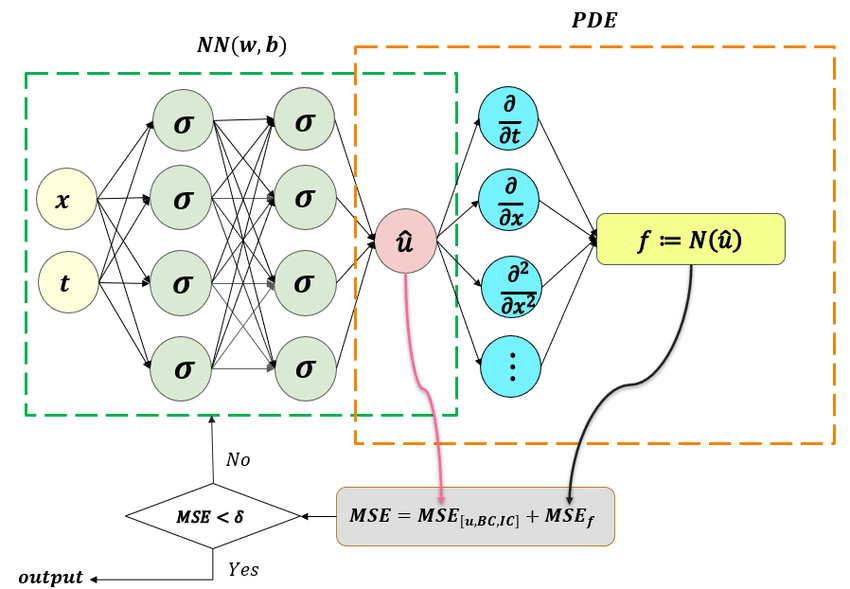
\includegraphics[scale=0.25]{pinn-schematic.png}
        \caption{The schematic of \glspl{PINN} for solving \glspl{PDE} \cite{guoSolvingPartialDifferential2020}.}
        \label{fig:pinn-schematic}
    \end{figure}
\end{frame}

\section{NeuralODEs}

\begin{frame}[fragile]{Neural ordinary differential equations: Idea}
    \begin{columns}
        \begin{column}{0.5\linewidth}
            \begin{figure}[h]
                \centering
                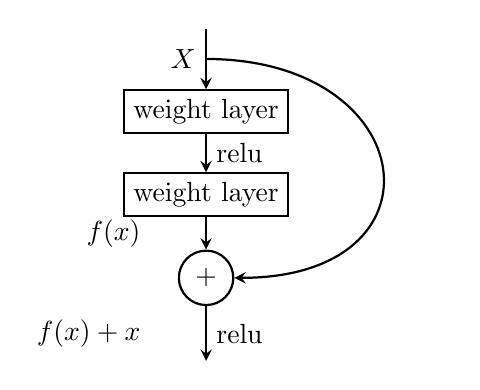
\begin{tikzpicture}[->, >=stealth, node distance = 3em, thick]
                    \tikzset{
                        block/.style  = {draw, thick, rectangle},
                        arith/.style  = {draw, thick, circle},
                        input/.style  = {coordinate},
                        output/.style = {coordinate}
                    }
                    \node[input] (IN) {};
                    \node[block, below of = IN] (W1) {weight layer};
                    \node[block, below of = W1] (W2) {weight layer};
                    \node[arith, below of = W2] (ADD) {+};
                    \node[output, below of = ADD] (OUT) {+};

                    \draw[->] (IN) to node[left, name = X]{$X$} (W1);
                    \draw[->] (X) to [out = 0, in = 0, looseness = 2.5] (ADD);
                    \draw[->] (W1) to node[right]{relu} (W2);
                    \draw[->] (W2) to node[xshift = -2em, left]{$f(x)$} (ADD);
                    \draw[->] (ADD) to node[xshift = -2em, left]{$f(x) + x$} node[right]{relu} (OUT);
                \end{tikzpicture}
                \caption{Skip connection}
                \label{fig:residual-network-skip-connection}
            \end{figure}
        \end{column}
        \begin{column}{0.5\linewidth}
            \begin{block}<2->{Observation}
                \begin{equation*}
                    \begin{aligned}
                        h_{t+1} &= h_t + f(h_t, \theta_t)\\
                        \Leftrightarrow \frac{dh(t)}{dt} &= f(h(t), t, \theta)
                    \end{aligned}
                \end{equation*}
            \end{block}
        \end{column}
    \end{columns}
\end{frame}

\begin{frame}{Neural ordinary differential equations: Formulation}

    \begin{block}<1->{\glsfirst{NeuralODE} output}
        \begin{equation*}
            z(t_1) = z(t_0) + \int_{t_0}^{t_1}{f(z(t), t, \theta)dt}
        \end{equation*}
    \end{block}

    \begin{itemize}
        \item<2-> Memory efficiency
        \item<3-> Adaptive computation
        \item<4-> Scalable and invertible normalizing flows
        \item<5-> Continuous time series models
    \end{itemize}
\end{frame}

\begin{frame}{Neural ordinary differential equations: Outputs}
    \begin{figure}[h]
        \centering
        \subcaptionbox{ResNet}{
            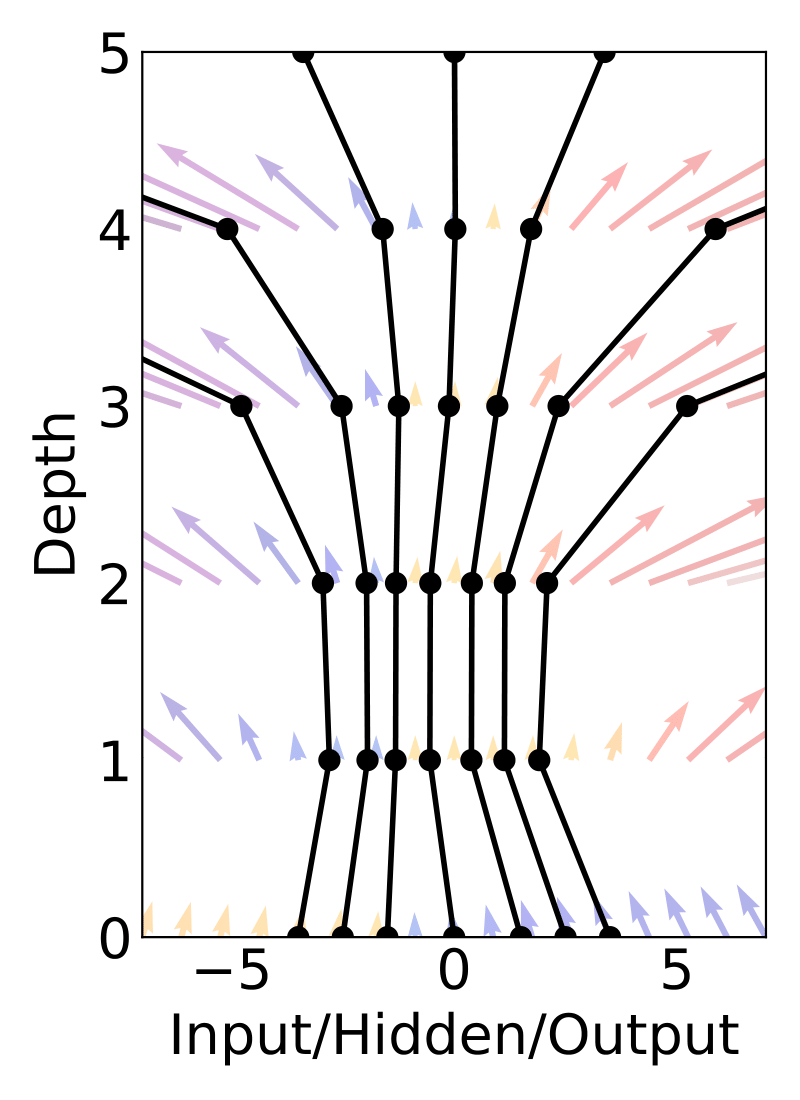
\includegraphics[scale=0.1]{neuralode_resnet.png}
        }
        \subcaptionbox{NeuralODE}{
            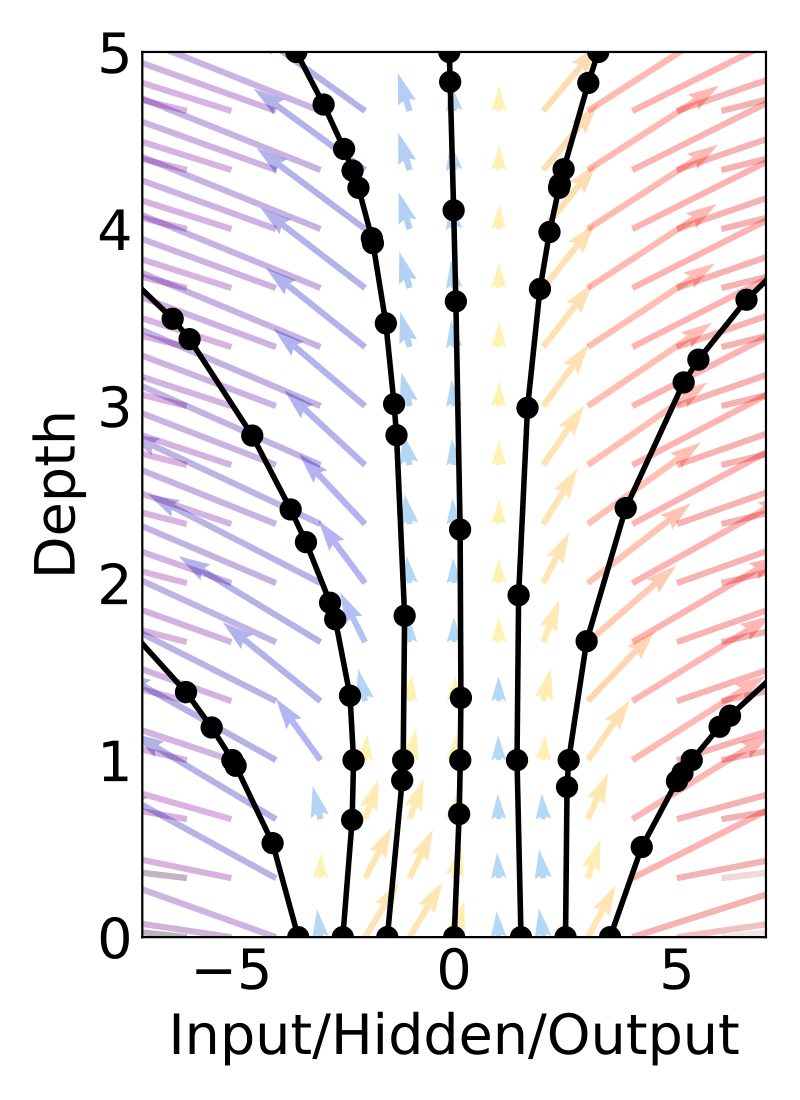
\includegraphics[scale=0.1]{neuralode_odenet.png}
        }
        \caption{Comparison between ResNet's discrete state transformations and \gls{NeuralODE} continuous state transformations}
        \label{fig:resnet-vs-odenet}
    \end{figure}
\end{frame}

\begin{frame}{Neural ordinary differential equations: Gradients}
    \begin{figure}[h]
        \centering
        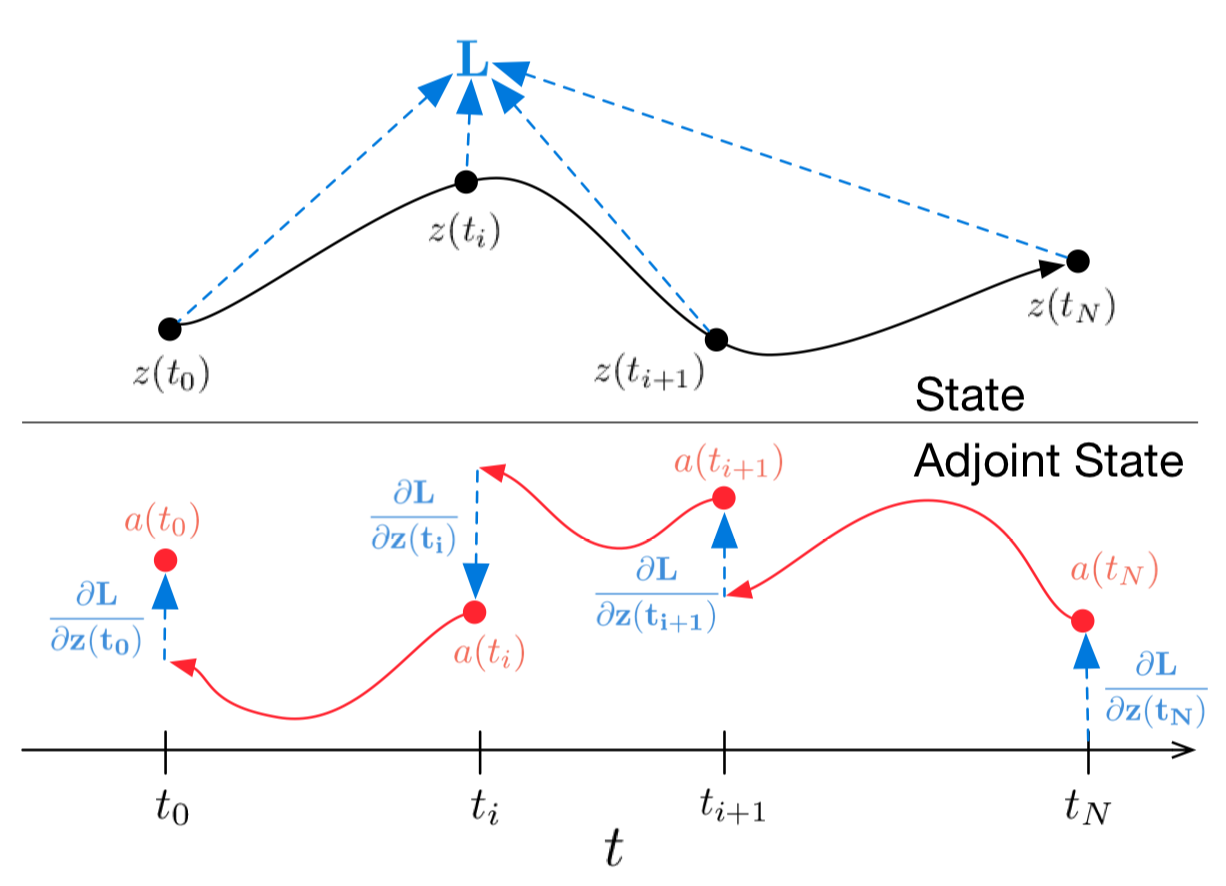
\includegraphics[scale=0.35]{neuralode-adjoint.png}
        \caption{Reverse-mode differentiation of an \gls{ODE} solution. \cite{chenNeuralOrdinaryDifferential2019}}
        \label{fig:neuralode-adjoint}
    \end{figure}
\end{frame}

\section{Software and hardware}

\begin{frame}{Software and hardware}
    Julia programming language
    \begin{itemize}
        \item \textit{DifferentialEquations} package
        \item \textit{DiffEqFlux} package
    \end{itemize}

    Linux systems
    \begin{itemize}
        \item Google Cloud Compute \textit{n2-standard-8} instance
        \item Personal laptop with 2-core \textit{Intel(R) Core(TM) i5-4260U} CPU 1.40GHz, and 4Gb of memory.
    \end{itemize}
\end{frame}

\begin{frame}[fragile]{Julia example}
\begin{figure}[!htb]
\centering
\begin{jllisting}
function SEIRD!(du, u, p, t)
    @inbounds begin
        S, E, I, _, _, N, C, _ = u
        β, γ, λ, α = p
        du[1] = -β * S * I / N
        du[2] = β * S * I / N - γ * E
        du[3] = γ * E - λ * I
        du[4] = (1 - α) * λ * I
        du[5] = α * λ * I
        du[6] = -α * λ * I
        du[7] = -C + γ * E
        du[8] = γ * E
    end
    return nothing
end
\end{jllisting}
\caption{Implementation of the system of ODEs in Julia}
\label{fig:diffeq-seird-inplace}
\end{figure}
\end{frame}

\section{Hyperparameters}

\begin{frame}{Hyperparameters}
    \begin{itemize}
        \item<1-> Initial time span of 4 days
        \item<1-> Time span increment of 4 days
        \item<2-> Time weighting parameter $\zeta = -0.001$
        \item<3-> ADAM optimizer
        \begin{itemize}
            \item Learning rate 0.05
            \begin{itemize}
                \item decay rate 0.5
                \item decay step 1000
                \item decay limit 0.00001
            \end{itemize}
            \item 1000 iterations on each time span
        \end{itemize}
        \item<4-> BFGS optimizer
        \begin{itemize}
            \item \textit{Initial stepnorm} 0.01
            \item 1000 iterations on the full time span
        \end{itemize}
    \end{itemize}
\end{frame}

\section{$R_0$ and fatality rate}

\begin{frame}{$R_0$ and fatality rate: Country-level data}
    \begin{figure}[!htb]
        \centering
        \subcaptionbox{Viet nam}{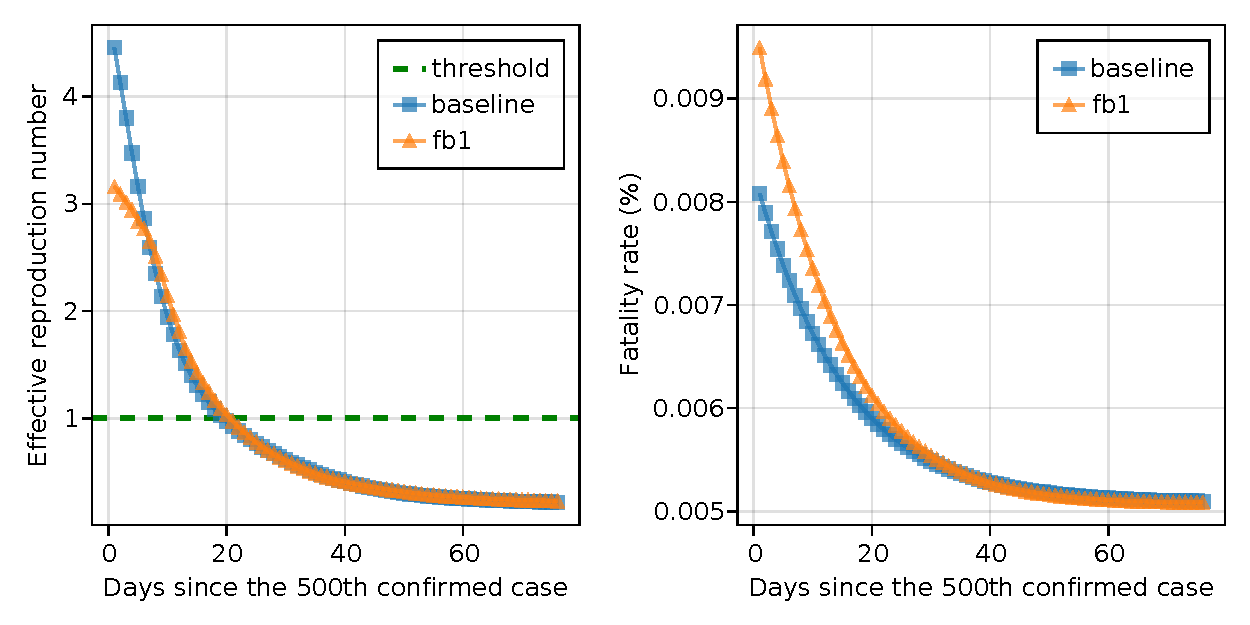
\includegraphics[width=0.45\linewidth]{Re_and_fatality_vietnam.pdf}}
        \subcaptionbox{United States}{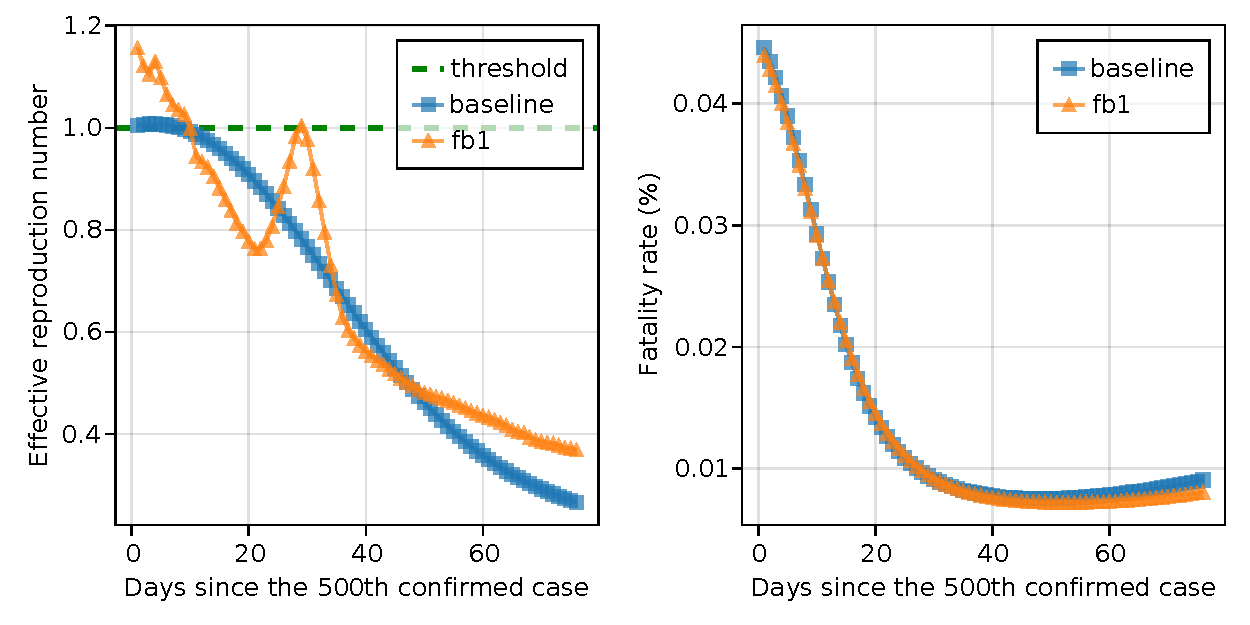
\includegraphics[width=0.45\linewidth]{Re_and_fatality_unitedstates.pdf}}
        \caption{Disease metrics learned by different versions of the model}
    \end{figure}
\end{frame}

\begin{frame}{$R_0$ and fatality rate: Counties in the United States}
    \begin{figure}[!htb]
        \centering
        \subcaptionbox{Harris, TX}{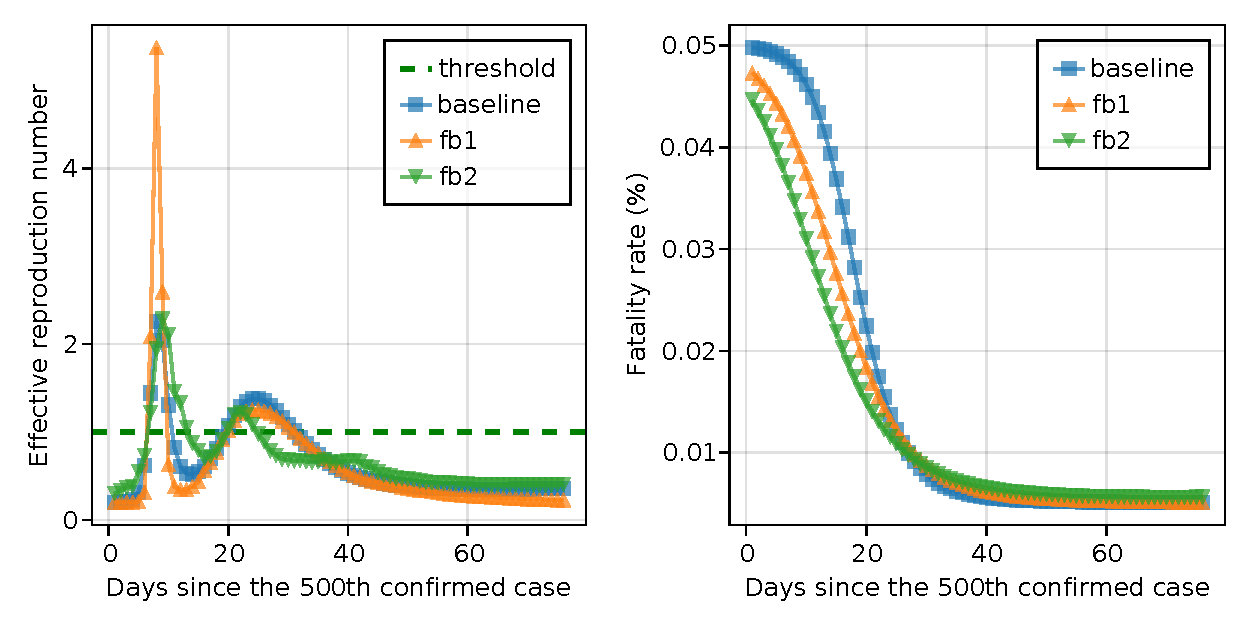
\includegraphics[width=0.45\linewidth]{Re_and_fatality_harris_tx.pdf}}
        \subcaptionbox{Los Angeles, CA}{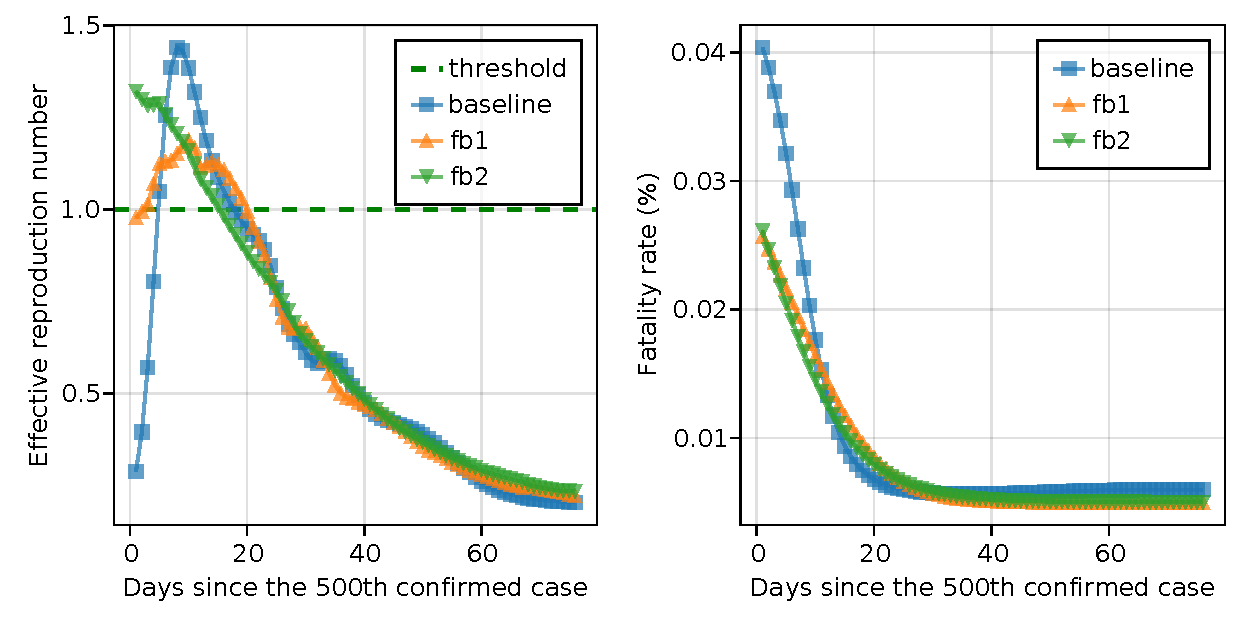
\includegraphics[width=0.45\linewidth]{Re_and_fatality_losangeles_ca.pdf}}
        \subcaptionbox{Maricopa, AZ}{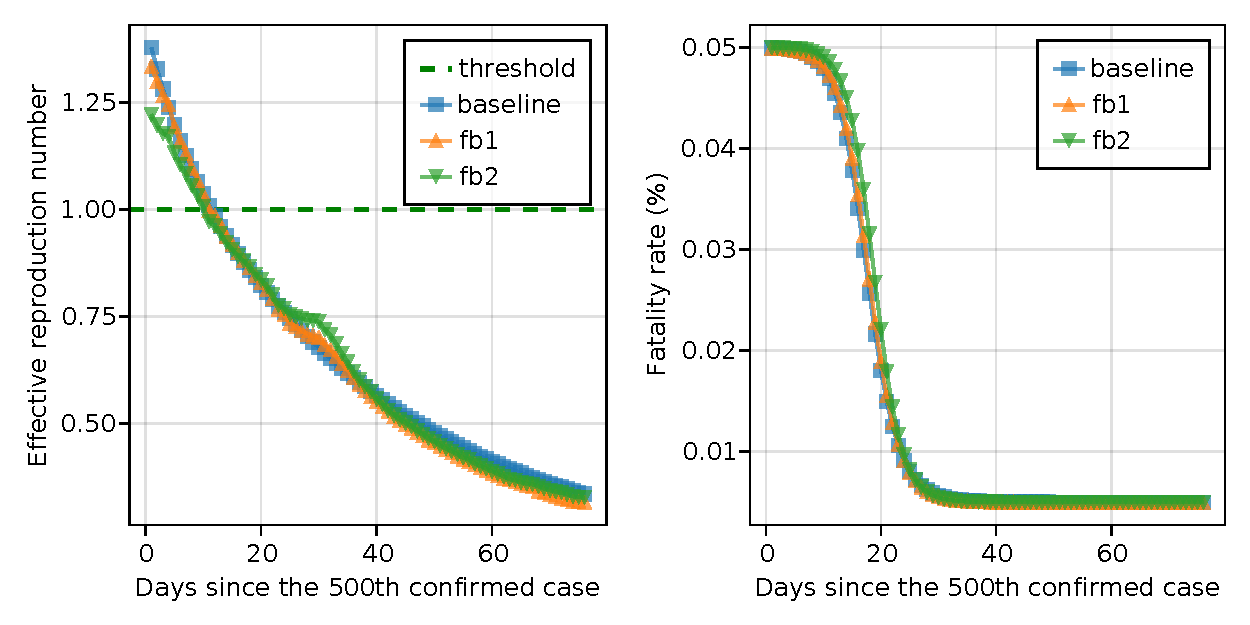
\includegraphics[width=0.45\linewidth]{Re_and_fatality_maricopa_az.pdf}}
        \subcaptionbox{Cook, IL}{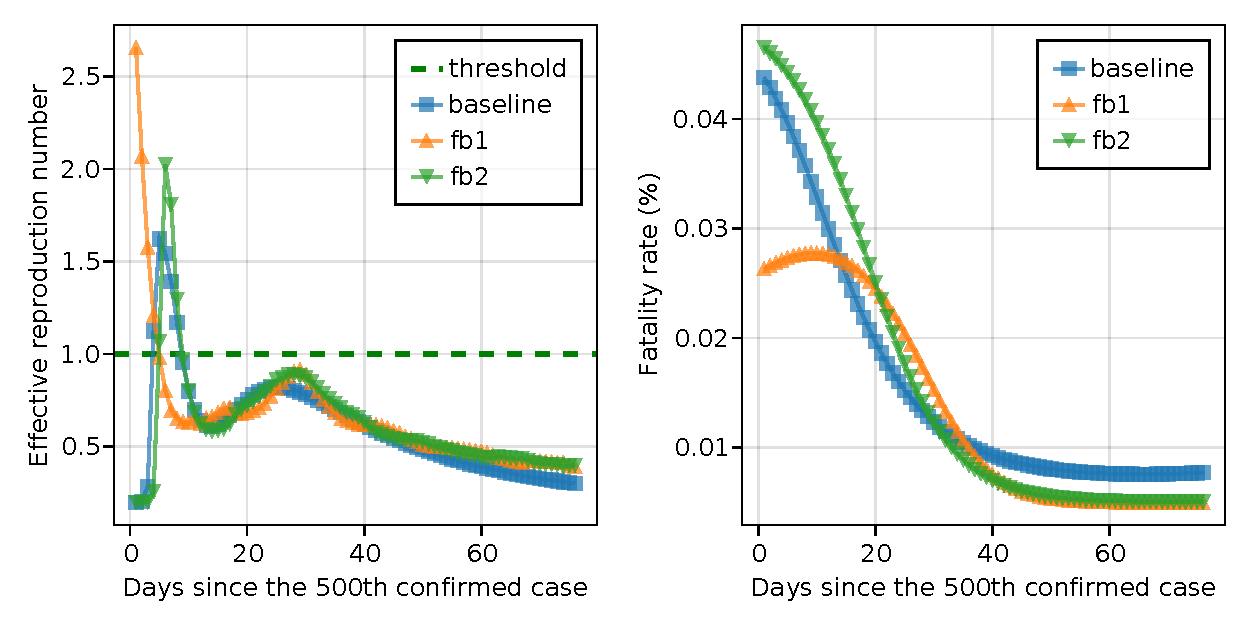
\includegraphics[width=0.4\linewidth]{Re_and_fatality_cook_il.pdf}}
        \caption{Disease metrics learned by different versions of the model}
    \end{figure}
\end{frame}

\begin{frame}{$R_0$ and fatality rate: Provinces in Vietnam}
    \begin{figure}[!htb]
        \centering
        \subcaptionbox{Dong Nai}{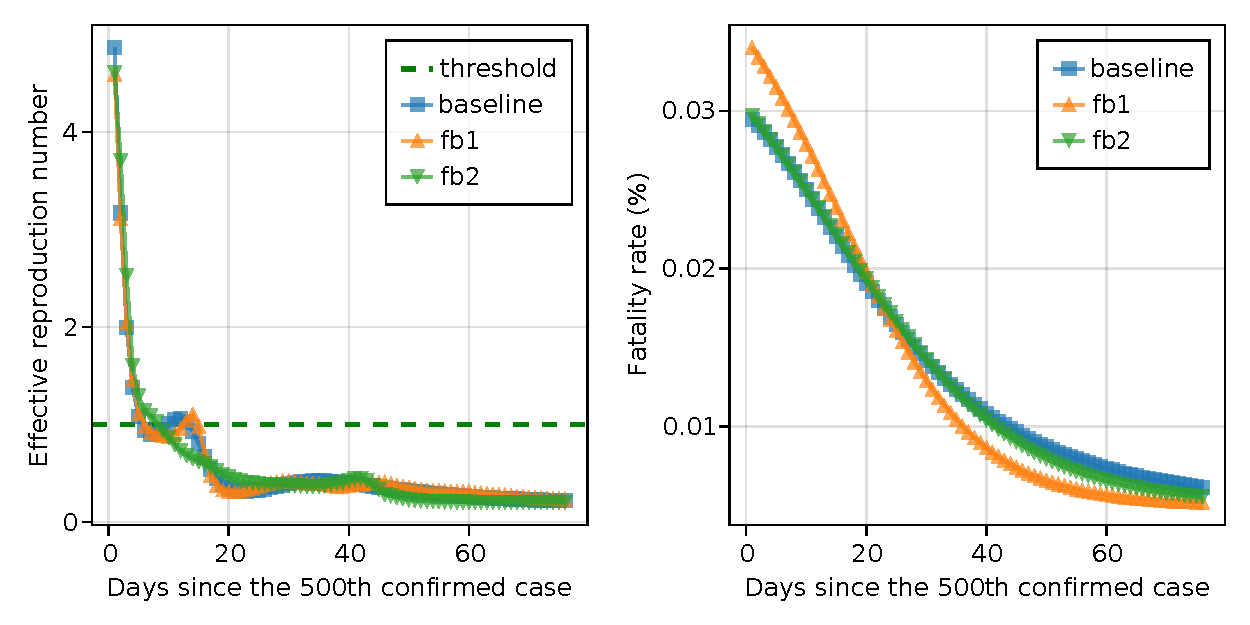
\includegraphics[width=0.45\linewidth]{Re_and_fatality_dongnai.pdf}}
        \subcaptionbox{Long An}{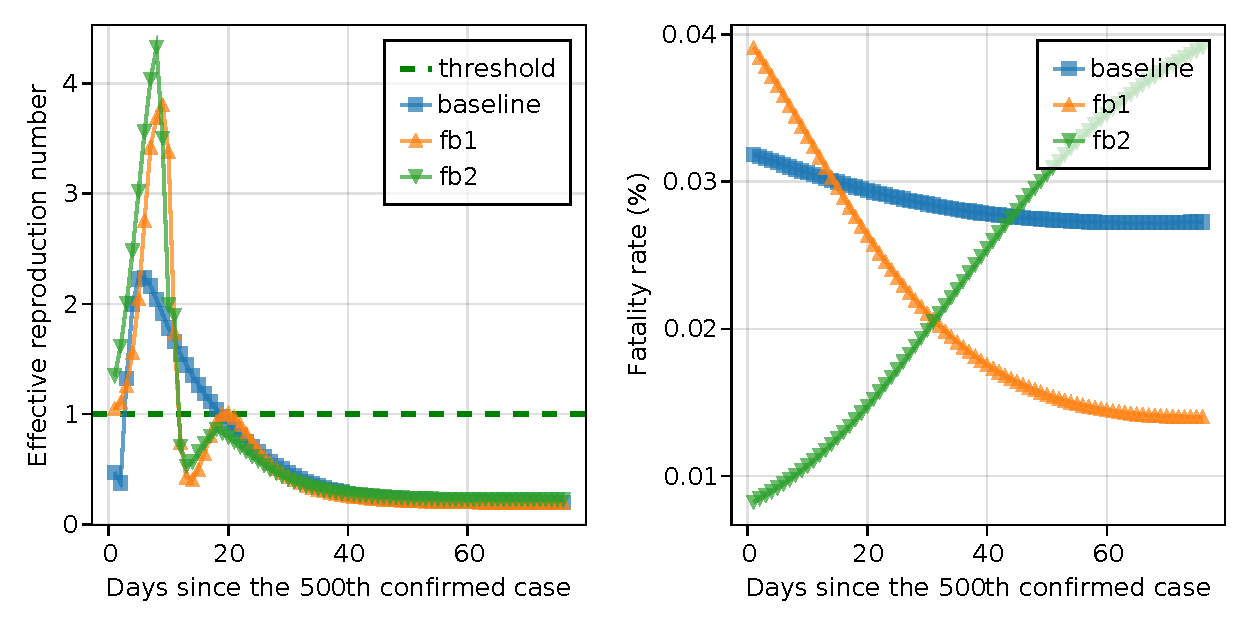
\includegraphics[width=0.45\linewidth]{Re_and_fatality_longan.pdf}}
        \subcaptionbox{Binh Duong}{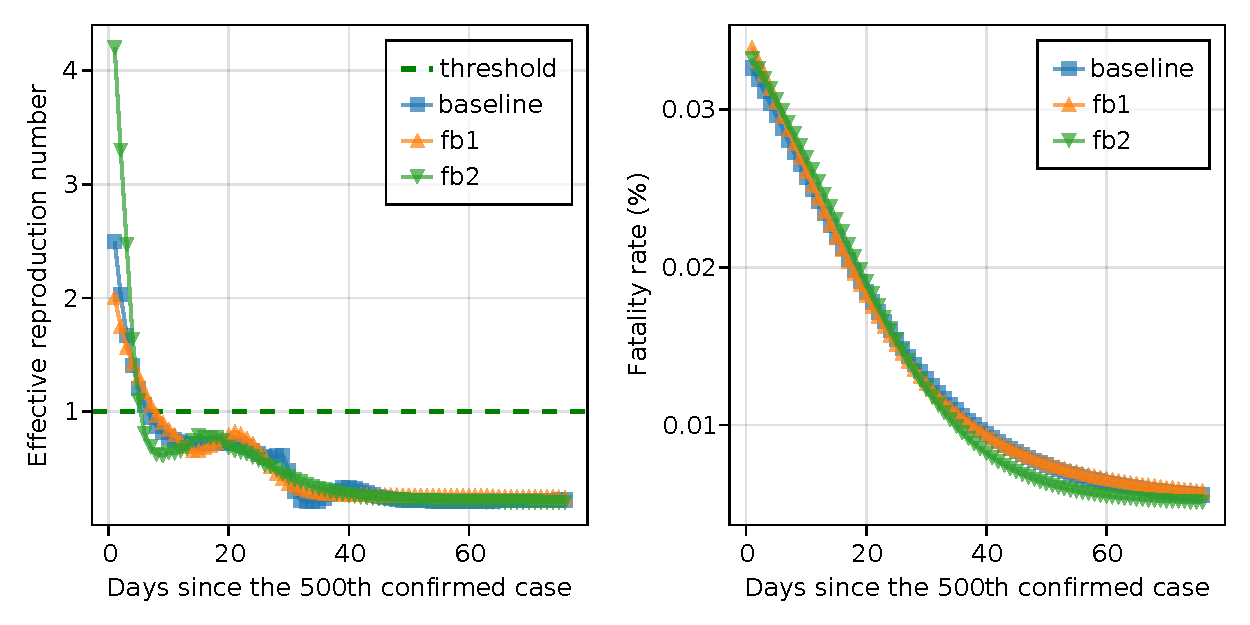
\includegraphics[width=0.45\linewidth]{Re_and_fatality_binhduong.pdf}}
        \subcaptionbox{Ho Chi Minh city}{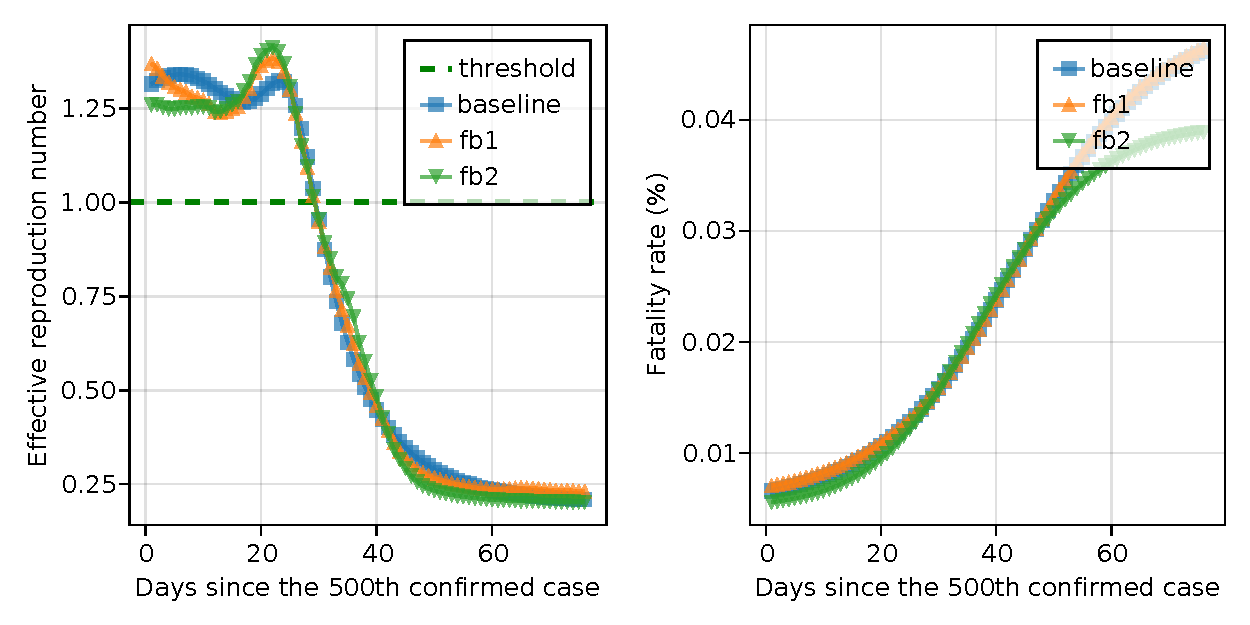
\includegraphics[width=0.45\linewidth]{Re_and_fatality_hcm.pdf}}
        \caption{Disease metrics learned by different versions of the model}
    \end{figure}
\end{frame}